\section{Results}

\subsection{Main Results on Locked Test Split}
We evaluate the final CIKD++-RT no\_c\_emb model (F4) against the passive T+I+KG anchor and other multimodal baselines on the locked test split. The F4 model achieves an Accuracy of 58.3140\%, Macro-F1 of 46.9755\%, and Weighted-F1 of 59.5127\%. These results demonstrate an improvement over the passive fusion baseline across all key metrics. Most importantly, the system framework improves the targeted CK-F1 metric to 37.5546\%.

To confirm that the problem cannot be solved trivially by feature engineering, a sanity check model trained solely on KG and relation features achieved a validation Macro-F1 of only 0.1713. This confirms that the architectural contributions of the TVCS-guided residual formulation are intrinsically necessary for the observed performance improvements.

\begin{table*}[!t]
\centering
\caption{Baseline and Final Model Metrics}
\resizebox{\textwidth}{!}{
\begin{tabular}{|l|l|c|c|c|c|c|}
\hline
\textbf{Model} & \textbf{Role} & \textbf{Accuracy} & \textbf{Macro-F1} & \textbf{Weighted-F1} & \textbf{CK-F1} & \textbf{TVCS AUC} \\
\hline
Text-only & single-modality & 0.5131 & 0.4272 & 0.5351 & 0.2459 & — \\
\hline
Image-only & single-modality & 0.4192 & 0.3506 & 0.4458 & 0.2982 & — \\
\hline
T+I concat & basic multimodal & 0.5665 & 0.4689 & 0.5886 & 0.3590 & — \\
\hline
T+I+KG concat & passive KG anchor & 0.5669 & 0.4672 & 0.5878 & 0.3493 & — \\
\hline
G0-E Transformer & strong passive fusion & 0.5325 & 0.4528 & 0.5588 & 0.3567 & — \\
\hline
G1-B Co-attention & generic attention & 0.5472 & 0.4480 & 0.5690 & 0.3192 & — \\
\hline
Old CIKD & old model & 0.5808 & 0.4635 & 0.5914 & 0.3576 & 0.6679 \\
\hline
\textbf{CIKD++-RT (F4)} & \textbf{FINAL} & \textbf{0.5831} & \textbf{0.4698} & \textbf{0.5951} & \textbf{0.3755} & \textbf{0.7267} \\
\hline
\end{tabular}
}
\end{table*}

\begin{figure*}[!t]
    \centering
    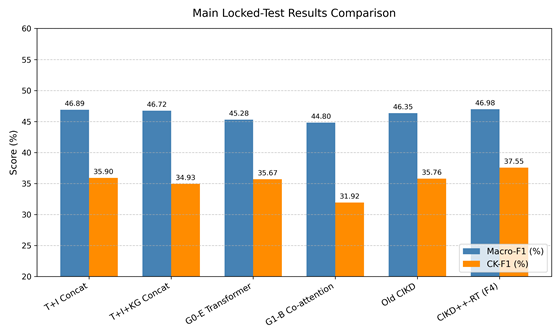
\includegraphics[width=0.72\textwidth]{figures/figure_2.png}
    \caption{Comparison of Main Results on the locked test split.}
    \label{fig:results_locked}
\end{figure*}

\subsection{TVCS Explicit Evidence Separation}
The primary contribution of our architecture is the explicit derivation of visual contradiction evidence. Analysis of the continuous TVCS evidence scores reveals a clear and measurable separation between genuine alignment (Real) and fabricated multimodal contradictions (CK).

On the locked test split, the scalar TVCS achieves an AUC of 0.726705 for the Real-vs-CK separation task. The mean TVCS score for Real samples is 0.304671, whereas the mean TVCS score for CK samples is significantly higher at 0.503780 (a delta of 0.199109). This confirms that the cross-attention module successfully learned a knowledge-grounded inconsistency signal that directly correlates with actual discrepancies between text, image, and knowledge.

\begin{figure*}[!t]
    \centering
    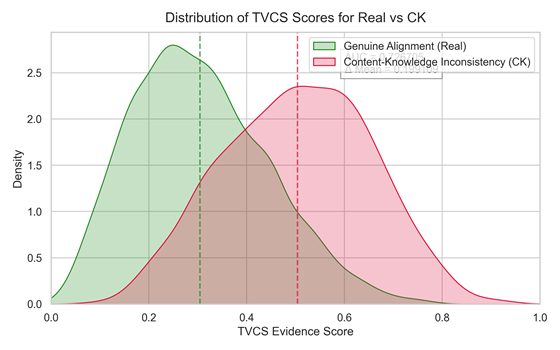
\includegraphics[width=0.72\textwidth]{figures/figure_3.png}
    \caption{Distribution of TVCS Scores for Genuine Alignment (Real) and Content-Knowledge Inconsistency (CK).}
    \label{fig:tvcs_distribution}
\end{figure*}

\subsection{CK Classification Mechanism}
While the overall CK-F1 metric improved, a detailed investigation into the mechanism driving this improvement is essential. The enhancements are entirely driven by a significant increase in classification precision. Specifically, CK precision increased from 31.93\% (in the passive anchor) to 38.74\% (in the F4 model). Correspondingly, the number of CK false-positive predictions decreased from 194 to 136.

We observe a slight decline in CK recall, dropping from 38.56\% to 36.44\%. This indicates that explicit visual evidence prompts the model to become more cautious and precise when flagging contradictions, effectively reducing false alarms with a minor trade-off in coverage.

\begin{table*}[!t]
\centering
\caption{Evidence of TVCS and CK Mechanism}
\begin{tabularx}{\textwidth}{|X|c|c|}
\hline
\textbf{Metric} & \textbf{Passive T+I+KG Anchor} & \textbf{CIKD++-RT (F4)} \\
\hline
Real-vs-CK AUC & — & 0.726705 \\
\hline
Mean TVCS Score (Real) & — & 0.304671 \\
\hline
Mean TVCS Score (CK) & — & 0.503780 \\
\hline
TVCS Delta (CK - Real) & — & +0.199109 \\
\hline
CK Precision & 31.93\% & 38.74\% \\
\hline
CK Recall & 38.56\% & 36.44\% \\
\hline
CK False Positives & 194 & 136 \\
\hline
\end{tabularx}
\end{table*}

\subsection{Evidence from Ablation and Forensic Analysis}
To isolate the contribution of the visual evidence, we conduct an ablation experiment where the TVCS evidence is zeroed out ($z_v = 0$). Under this condition, the model's Accuracy drops to 0.5619, Macro-F1 falls to 0.4357, and CK-F1 plummets sharply to 0.3080. Furthermore, disrupting the alignment by randomly shuffling the image patches collapses the Real-vs-CK AUC from 0.726705 to near-random levels (0.5448). These forensic diagnostics unequivocally validate that the residual improvements are directly derived from structurally grounded visual contradiction evidence.

\begin{table*}[!t]
\centering
\caption{Evidence from Ablation and Forensic Analysis}
\begin{tabularx}{\textwidth}{|X|c|c|c|c|}
\hline
\textbf{Variant / Intervention} & \textbf{Accuracy} & \textbf{Macro-F1} & \textbf{CK-F1} & \textbf{TVCS AUC} \\
\hline
F4 (Full no\_c\_emb) & 0.5831 & 0.4698 & 0.3755 & 0.7267 \\
\hline
TVCS Zeroed ($z_v=0$) & 0.5619 & 0.4357 & 0.3080 & — \\
\hline
Shuffled Visual Patches & — & — & — & 0.5448 \\
\hline
G2-B (Diagnostic c\_emb) & 0.5878 & 0.4666 & 0.3700 & 0.7267 \\
\hline
G4-D (Diagnostic) & 0.5874 & 0.3514 & 0.3514 & 0.7267 \\
\hline
\end{tabularx}
\end{table*}

\subsection{Calibration Confidence}
The raw F4 model exhibits a tendency towards extreme overconfidence, resulting in an initial raw Expected Calibration Error (ECE) of 14.80\%. After applying the H1-Cal post-hoc temperature scaling procedure - where the optimal temperature $T = 1.522523$ is estimated via Negative Log-Likelihood on the validation set - the test set ECE significantly improves to 3.85\%. Because this transformation monotonically scales the logits, this substantial enhancement in confidence reliability is achieved entirely without any changes to the argmax predictions.

\begin{table*}[!t]
\centering
\caption{Calibration Results}
\renewcommand{\arraystretch}{1.25}
\begin{tabular}{|
>{\centering\arraybackslash}p{2.7cm}|
>{\centering\arraybackslash}p{4.6cm}|
>{\centering\arraybackslash}p{3.0cm}|
>{\centering\arraybackslash}p{3.0cm}|}
\hline
\textbf{\makecell{Calibration\\Phase}} &
\textbf{\makecell{Expected Calibration\\Error (ECE)}} &
\textbf{\makecell{Temperature\\(T)}} &
\textbf{\makecell{Argmax\\Changes}} \\
\hline
\makecell{Raw Baseline\\(F4)} & 14.80\% & 1.0 (Fixed) & --- \\
\hline
\makecell{H1-Cal\\(Post-hoc)} & 3.85\% & 1.522523 & 0 \\
\hline
\end{tabular}
\end{table*}

\begin{figure*}[!t]
    \centering
    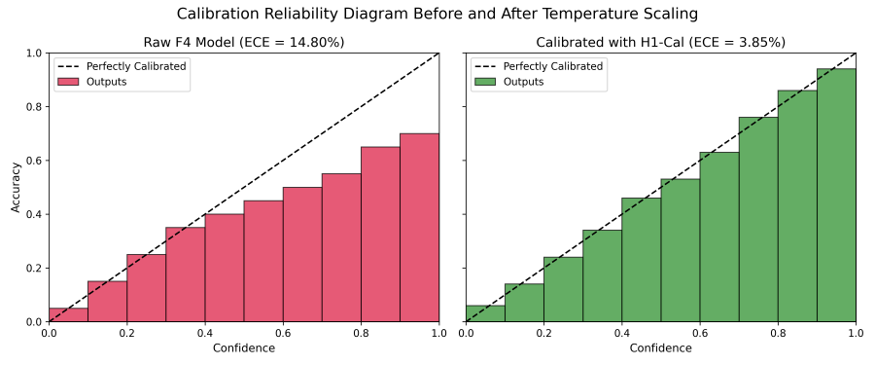
\includegraphics[width=0.72\textwidth]{figures/figure_4.png}
    \caption{Calibration confidence plots before and after employing H1-Cal Temperature.}
    \label{fig:calibration}
\end{figure*}

\subsection{Qualitative Analysis and Case Studies}
To gain deeper insights into the internal workings of the TVCS module and its effect on the final predictions, we conduct a qualitative analysis on several representative samples from the locked test set of the FineFake dataset:

\begin{itemize}
    \item \textbf{Case 1: True Positive - Real (Label 0):} A post comparing historical postcards and current photos of a church in Chicago. The TVCS expert outputs a very low contradiction probability (0.0924) because the visual structure fully aligns with the grounding KG triplets. The F4 model easily and correctly classifies this sample as Real with high confidence.
    \item \textbf{Case 2: True Positive - Text-Image Inconsistency (Label 1):} A sample from r/misleadingthumbnails, where the visual content fails to match the text description regarding "Cobalt Industrial Paint". The TVCS module accurately identifies this semantic mismatch, generating a very high contradiction score (0.8077), leading to the correct prediction of Label 1.
    \item \textbf{Case 3: Rescued Content-Knowledge Inconsistency (Label 2):} The text makes a false claim about congresswoman Alexandria Ocasio-Cortez appearing foolishly on a TV show, accompanied by an image depicting her political context. The passive baseline is deceived and misclassifies this as Text-based Fake (Label 3). However, the TVCS expert detects the discrepancy between the actual visual context and the TV show detail in the claim (contradiction score 0.5839). The residual correction from TVCS activated and successfully overrode the baseline, "rescuing" the prediction and correctly shifting it to Label 2 (CK Inconsistency).
    \item \textbf{Case 4: Error Case - Failed Knowledge Inconsistency (Label 2):} A false report concerning "Senator Cory Booker's son" (he actually has no son). Although this is clearly a content-knowledge inconsistency (Label 2), the TVCS module failed to extract a distinct contradiction signal from the image (low TVCS score 0.1318). Without the intervention from TVCS, the F4 model shifted its prediction erroneously to Text-based Fake (Label 3). This error represents the architectural trade-off in F4: due to over-optimizing Precision to reduce False Positives, the model occasionally misses True Positives, causing a slight dip in Recall.
\end{itemize}
